\section{Part 1}\label{sec:01_part1}

\subsection{Introduction}\label{subsec:01_part1_intro}
% Intro to the HTTP server
In the second lecture of the course, an implementation of a basic HTTP server with the name \textit{TinyHttpd} was introduced.
The functionality of \textit{TinyHttpd} is limited to opening \texttt{.html} files and delivering the content via the HTTP 1.1 protocol to the client.


% Problem statement
The task of part 1 of the first assignment, is to extend the \textit{TinyHttpd} implementation by implementing the functionality to launch an external process. Therefore, the client sends a request via the URL \path{http://localhost:8000/process/reverse?par1=ROMA}. Then, the server executes an external Java process, which reverses the string \texttt{ROMA}, given in the query \texttt{?par1=ROMA}, and responses the result (\texttt{AMOR}) of the external Java process to the client via HTTP 1.1.


% Domain description
Given the above-mentioned task description, the following steps have to be implemented:
\begin{enumerate}
\item Create a Java application, called \textit{StringReverser}, which takes a valid String as input and returns the reversed string
\item Extend the \textit{TinyHttpd} implementation to launch external processes when requested by the client via the URL \path{http://localhost:8000/process/PROCESS_NAME?PROCESS_PARAMETERS}.
\item Execute the requested process on the server and deliver the process output to the client via the HTTP protocol.
\end{enumerate}


\newpage
\subsection{Conceptual Design}\label{subsec:01_part1_design}
Given the problem statement introduced in \Sec{subsec:01_part1_intro}, a new application called \textit{StringReverser} needs to be implemented, and the \textit{TinyHttpd} server has to be extended in a way to launch an external Java process.

\subsubsection{StringReverser}\label{subsubsec:01_part1_design_stringreverser}
% Design of the StringReverser
The \textit{StringReverser} application is a simple terminal application. It takes any valid String as an input and returns the reversed string as the output. It can be executed via the console. For example, the command \texttt{\$ java -jar StringReverser.jar ROMA} should responses the string \textit{AMOR}.

\subsubsection{TinyHttpd}\label{subsubsec:01_part1_design_tinyhttpd}
% Extension of TinyHttpd
Whenever the client requests the URL \path{http://localhost:8000/process/PROCESS_NAME?PROCESS_PARAMETERS}, the server is supposed to start an external Java process, waits for the output of the process, and responses the process output to the user.
% URL
The client can specify which process has to be executed. Given the URL \path{http://localhost:8000/process/reverse?par1=ROMA}, the user explicitly requests to launch the \textit{reverse} process with the given query \texttt{par1=ROMA} as the process input.
% Input
It is important to mention, that each process takes individual parameters as input. For the above-mentioned \texttt{StringReverser}, only the value of the first parameter in the given query is important. All other parameters, and the parameter key, are therefore ignored.


\newpage
\subsection{Implementation}\label{subsec:01_part1_impl}
To implement the given conceptual design mentioned in \Sec{subsec:01_part1_design}, OpenJDK 17\footnote{JDK 17 - \url{https://openjdk.java.net/projects/jdk/17/} (Accessed: 02/10/2021)} is used.

\subsubsection{StringReverser}\label{subsubsec:01_part1_impl_stringreverser}
% Implementation of StringReverser
The application \textit{StringReverser} is a simple Java project. It is composed of a single Java class called \texttt{StringReverser} as shown in \Fig{fig:01_part1_impl_stringreverser_structure}.
% Implementation of StringReverser
The source code is shown in \Lst{lst:01_part1_impl_stringreverser_code}, and it consists of a \texttt{main} method and a method called \texttt{reverseString}.
% The main method
The main method will be executed, when the application is launched via the terminal. Additionally, it checks if the given input string is valid. Otherwise, it will return an error message and exit with system code 0. If the input is a valid string, it will call the \texttt{reverseString} method, and returns the result as the output.
% The reverse method
The \texttt{reverseMethod} is responsible to reverse the given input. To achieve this, it uses the \texttt{StringBuilder}\footnote{StringBuilder - \url{https://docs.oracle.com/javase/7/docs/api/java/lang/StringBuilder.html} (Accessed: 02/10/2021)} class to reverse the String.

% StringReverser project structure
\begin{figure}[h]
\centering
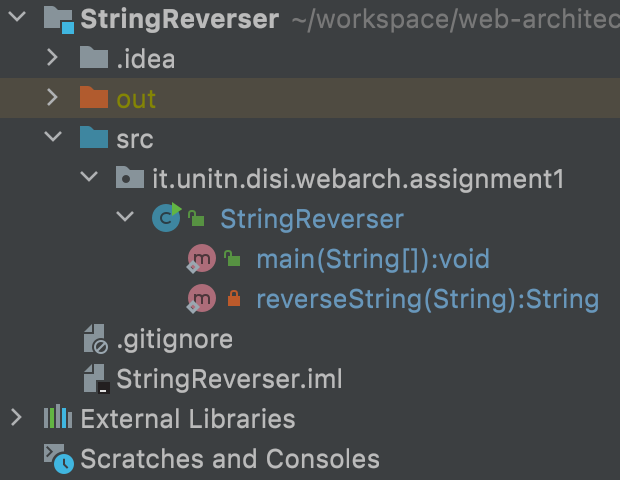
\includegraphics[scale=0.4]{images/StringReverserStrct}
\caption{Project structure of the \texttt{StringReverser} application}
\label{fig:01_part1_impl_stringreverser_structure}
\end{figure}

% Execution
\Fig{fig:01_part1_impl_stringreverser_execution} shows the execution of the \textit{StringReverser} application. The \texttt{.jar} artifact was created using the IntelliJ IDEA\footnote{Create your first Java application - \url{https://www.jetbrains.com/help/idea/creating-and-running-your-first-java-application.html} (Accessed: 02/10/2021)}.
% Failure execution
If the input is invalid, the \texttt{StringReverser} will print an error message to the terminal and exit with system code 0, as shown in \Fig{fig:01_part1_impl_stringreverser_execution_fail}.

% StringReverser execution
\begin{figure}[h]
\centering
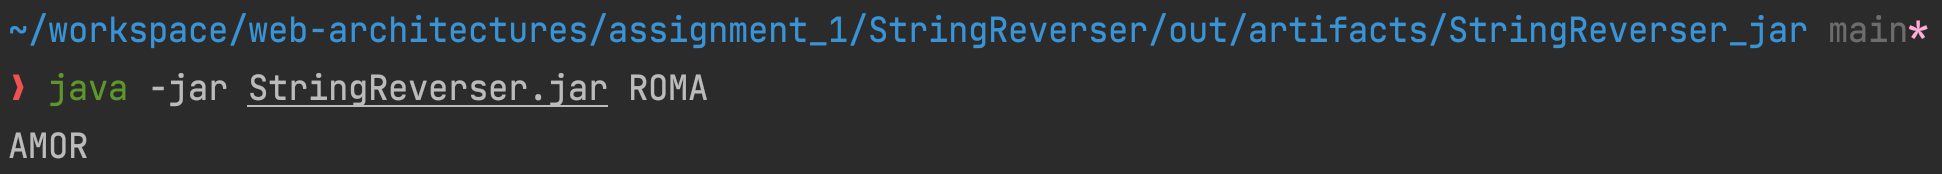
\includegraphics[scale=0.4]{images/StringReverserExec}
\caption{Successful execution of the \textit{StringReverser} application}
\label{fig:01_part1_impl_stringreverser_execution}
\end{figure}

% StringReverser execution fail
\begin{figure}[h]
\centering
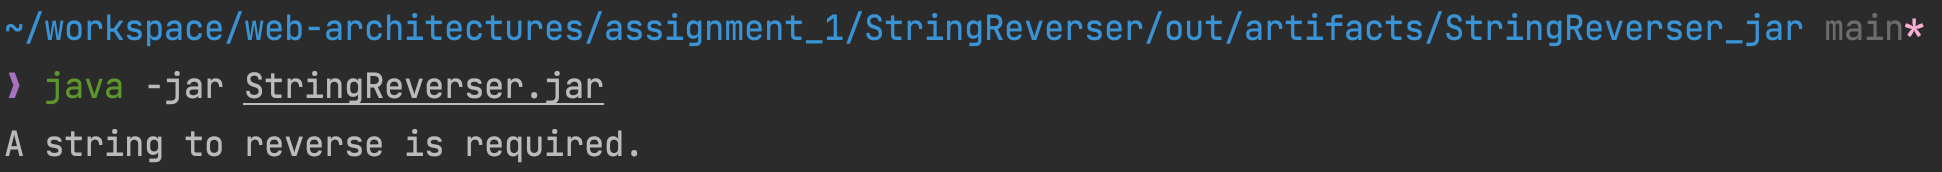
\includegraphics[scale=0.4]{images/StringReverserExecFail}
\caption{Execution of the \textit{StringReverser} application without an input}
\label{fig:01_part1_impl_stringreverser_execution_fail}
\end{figure}

\subsubsection{TinyHttpd}
% Extension of TinyHttpd
The foundation of the \textit{TinyHttpd} project is provided by the Professor. It has to be extended to launch an external Java process and deliver the process output to the client as an HTTP response.
% The steps
To implement the conceptual design mentioned in \Sec{subsubsec:01_part1_design_tinyhttpd}, the \textit{TinyHttpd} project has to be extended in the following way:
% impl details
\begin{enumerate}
\item Parse the HTTP request to check if a process has been requested
\item Generate the command to execute the requested process
\item Launch an external process, using the generated command
\item Response the process output to the client via HTTP
\end{enumerate}
In the following, the single steps are described in detail.


% Parse request
\paragraph{Step 1:}
The first step of the implementation, is to check if the client's requested the execution of a process. Therefore, the HTTP request has to be parsed accordingly. For this task, a new Java class called \texttt{RequestParser} is introduced to the \textit{TinyHttpd} project. The \texttt{RequestParser} class can parse an HTTP request into its parts. For example, the request \texttt{GET /process/reverse?param=roma HTTP/1.1} is composed of the HTTP method (\texttt{GET}), the path (\path{/process/reverse?param=roma}), and the HTTP protocol version (\texttt{HTTP/1.1}). Furthermore, the path has an additional query attached (\texttt{?param=roma}). The implementation of the \texttt{RequestParser} class is attached at \Lst{lst:01_part1_impl_tinyhttpd_requestparser}.


% Then start process
After the \texttt{RequestParser} has successfully parsed the clients request, it is possible to check, by using an \texttt{if} statement, if the user requested the path \path{/request/PROCESS_NAME}. If yes, the server executes the requested process and sends a response accordingly. Otherwise, an error message is sent to the user as shown in \Fig{fig:01_part1_impl_tinyhttpd_invalidprocess}. If no process has been requested, the server tries to open the HTML file according to the given path and responds the HTML content to the client.

% Invalid process
\begin{figure}[h]
\centering
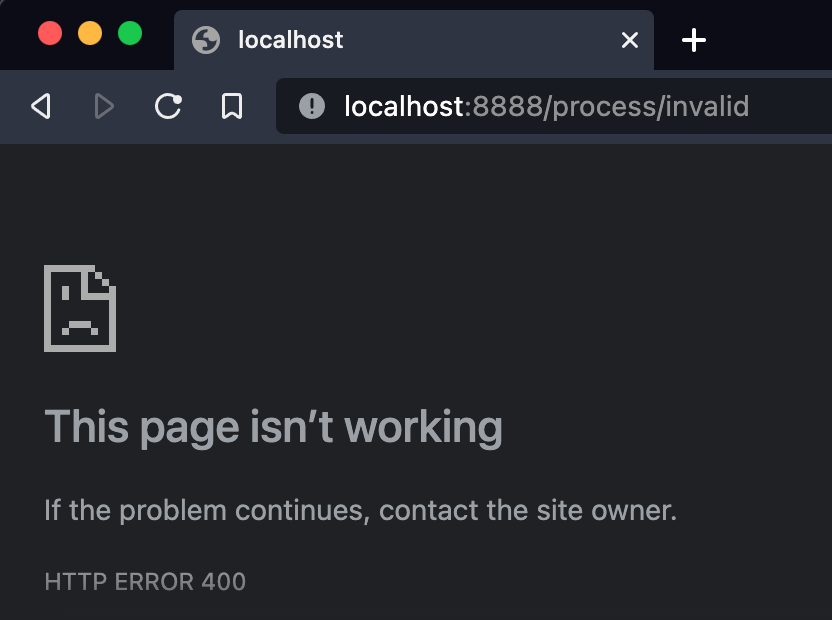
\includegraphics[scale=0.4]{images/invalidProcess}
\caption{Response for an invalid process name}
\label{fig:01_part1_impl_tinyhttpd_invalidprocess}
\end{figure}


% Start the requestes process
\paragraph{Step 2:}
If the client has sent a valid request for a process, the next step is to generate the command to launch the requested process. To keep the \textit{TinyHttpd} implementation extensible, a new class called \texttt{CommandFactory} is added to the project, which is implemented using the Factory pattern. The implementation of this class is attached at \Lst{lst:01_part1_impl_tinyhttpd_commandfactory}.
% CommandFactory
The \texttt{CommandFactory} class is responsible to generate the command for the given request. It has a public static method called \texttt{generateCommand}, which takes the requested process name and the query of the request path as arguments. If the given query is invalid, the method will throw an exception and an error message is sent to the client as seen in \Fig{fig:01_part1_impl_tinyhttpd_invalidquery}.
% Explain the method
According to the given process name, it generates the command to execute the \texttt{.jar} artifact with the given query as an input parameter.
% Example
As example, for the given path \texttt{/process/reverse?param=roma}, the generated command is \texttt{java -jar} \path{/Users/marcel/workspace/web-architectures/assignment_1/MiniHTTPD/jars/StringReverser.jar} \texttt{"roma"}. In addition, the \texttt{CommandFactory} is also responsible for checking, if the requested process is available and if the given query is a valid parameter for the process. If not, it will throw an exception.

% Invalid process
\begin{figure}[h]
\centering
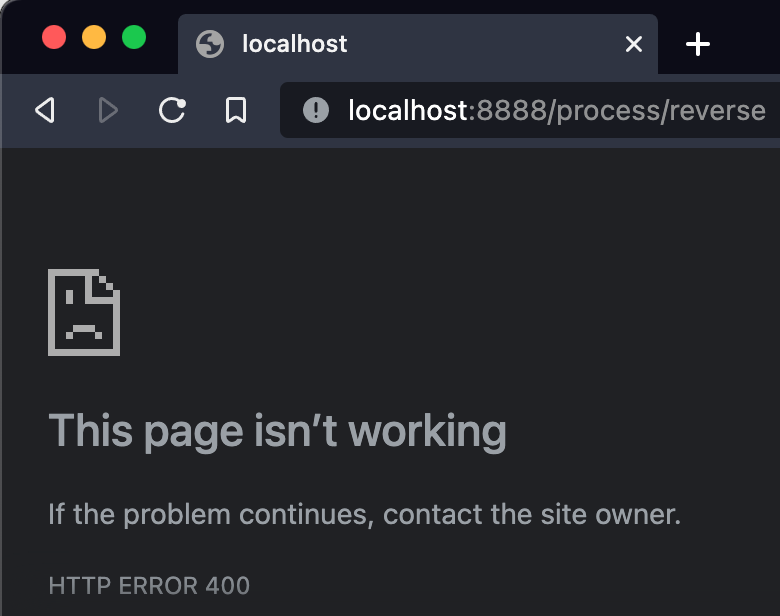
\includegraphics[scale=0.4]{images/invalidQuery}
\caption{Response for an invalid query}
\label{fig:01_part1_impl_tinyhttpd_invalidquery}
\end{figure}


% Launch process
\paragraph{Step 3:}
After the command has been generated, it needs to be executed in a shell. To achieve this, the \texttt{TinyHttpd} class is extended with a new method called \texttt{launchProcess}. The implementation of this method is available at \Lst{lst:01_part1_impl_tinyhttpd_launchprocess}. This method takes the generated command as an argument and executes it using the \texttt{ProcessBuilder}\footnote{ProcessBuilder - \url{https://docs.oracle.com/javase/7/docs/api/java/lang/ProcessBuilder.html} (Accessed: 02/10/2021)} class.
% How it is executed
The method executes the given command in the bash shell using \texttt{bash -c COMMAND} and returns the process output as a string. It is important, that the process output is returned as a string, instead of printing it directly to the HTTP output stream. The reason is, that the HTTP header of the server response needs the length of the process output.
% Show the execution
\Lst{lst:01_part1_impl_tinyhttpd_implsteps} shows the execution of the \texttt{launchProcess} method and \Fig{fig:01_part1_impl_output} shows the output to the console after the process has been executed successfully.

% steps implementation
\begin{figure}[h]
\centering
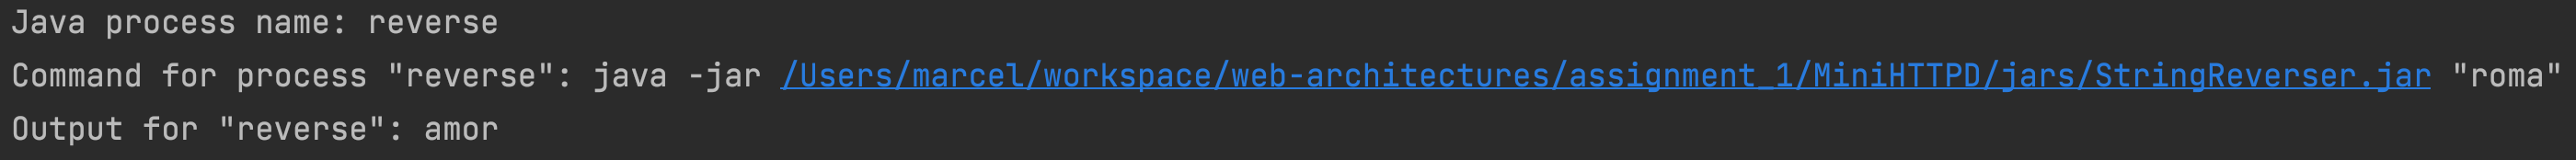
\includegraphics[scale=0.3]{images/implementationOutput}
\caption{Console output after the generated command has been launched successfully}
\label{fig:01_part1_impl_output}
\end{figure}


% Response to the client
\paragraph{Step 4:}
The last step, is to send the process output as an HTTP response to the client.
% How its send
A method called \texttt{sendSuccessResponseHeader} is added to the \textit{TinyHttpd} class, which is responsible to send a \texttt{200 OK} HTTP response. Additionally, the method takes the length of the output as an argument, which was mentioned before, as well as the MIME type of the response content. The implementation of the \texttt{sendSuccessResponseHeader} is attached at \Lst{lst:01_part1_impl_tinyhttpd_sendSuccessResponseHeader}.
% Send
\Lst{lst:01_part1_impl_tinyhttpd_implsteps} shows the whole process of generating the process command, launching the command, and sending the response to the client. First, a header with the process output length and the MIME type \texttt{text/plain} is written to the output stream, then the process output. \Fig{fig:01_part1_impl_success} shows the response in the browser for a successful process request.

% successful response
\begin{figure}[h]
\centering
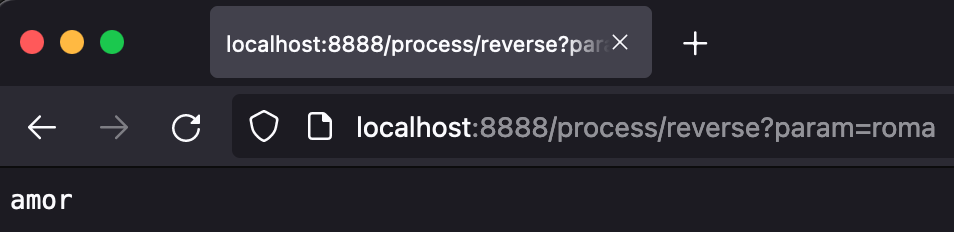
\includegraphics[scale=0.6]{images/part1Success}
\caption{A successful process request}
\label{fig:01_part1_impl_success}
\end{figure}
